
\documentclass[11pt]{article}

\usepackage[margin=1in]{geometry}
\usepackage{amsmath, amssymb, amsfonts}
\usepackage{graphicx}
\usepackage{float}
\usepackage{caption}
\usepackage{booktabs}
\usepackage{enumitem}
\usepackage{mathtools}
\usepackage{hyperref}
\usepackage{helvet}
\renewcommand{\familydefault}{\sfdefault}

\setlength{\parindent}{0in}

\graphicspath{{HW2/}}

\title{Homework 1: Working with Immersed Boundaries}
\author{}
\date{}

\begin{document}

\maketitle

% ==========================================================
\section*{Problem 1: Poisson Equation}
% ==========================================================

\textbf{Question.}
Solve the two-dimensional Poisson equation
\[
\nabla^2 u=f(x,y)
\]
on the square domain $[0,2\pi]^2$ using finite differences with Dirichlet boundary conditions. Choose the forcing function and boundary values such that
\[
u(x,y)=\cos(2x)\sin(2y)
\]
is the exact solution. Verify that the numerical method exhibits second-order convergence as the grid is refined.

\subsection*{Solution}

The forcing function is obtained by applying the Laplacian to the exact solution:
\[
f(x,y)=\nabla^2u=-8\cos(2x)\sin(2y).
\]
We approximate the Laplacian using the five-point finite-difference stencil:
\[
\nabla^2u_{i,j}\approx
\frac{
u_{i+1,j}+u_{i-1,j}+u_{i,j+1}+u_{i,j-1}
-4u_{i,j}
}{h^2}.
\]
This approximation has second-order accuracy.

We measure the numerical error using the relative $L^2$ norm:
\[
\mathrm{Err}_{\mathrm{rel},L^2}
=
\frac{\|u-u_n\|_2}{\|u\|_2}.
\]
This measures the numerical error relative to the magnitude of the exact solution.


\begin{table}[H]
\centering
\begin{tabular}{cc}
\toprule
$N$ & Relative $L^2$ Error\\
\midrule
20  & $2.936\times10^{-2}$\\
40  & $7.400\times10^{-3}$\\
80  & $1.865\times10^{-3}$\\
160 & $4.686\times10^{-4}$\\
\bottomrule
\end{tabular}
\caption{Relative $L^2$ error for increasing grid sizes.}
\end{table}

\begin{figure}[H]
\centering
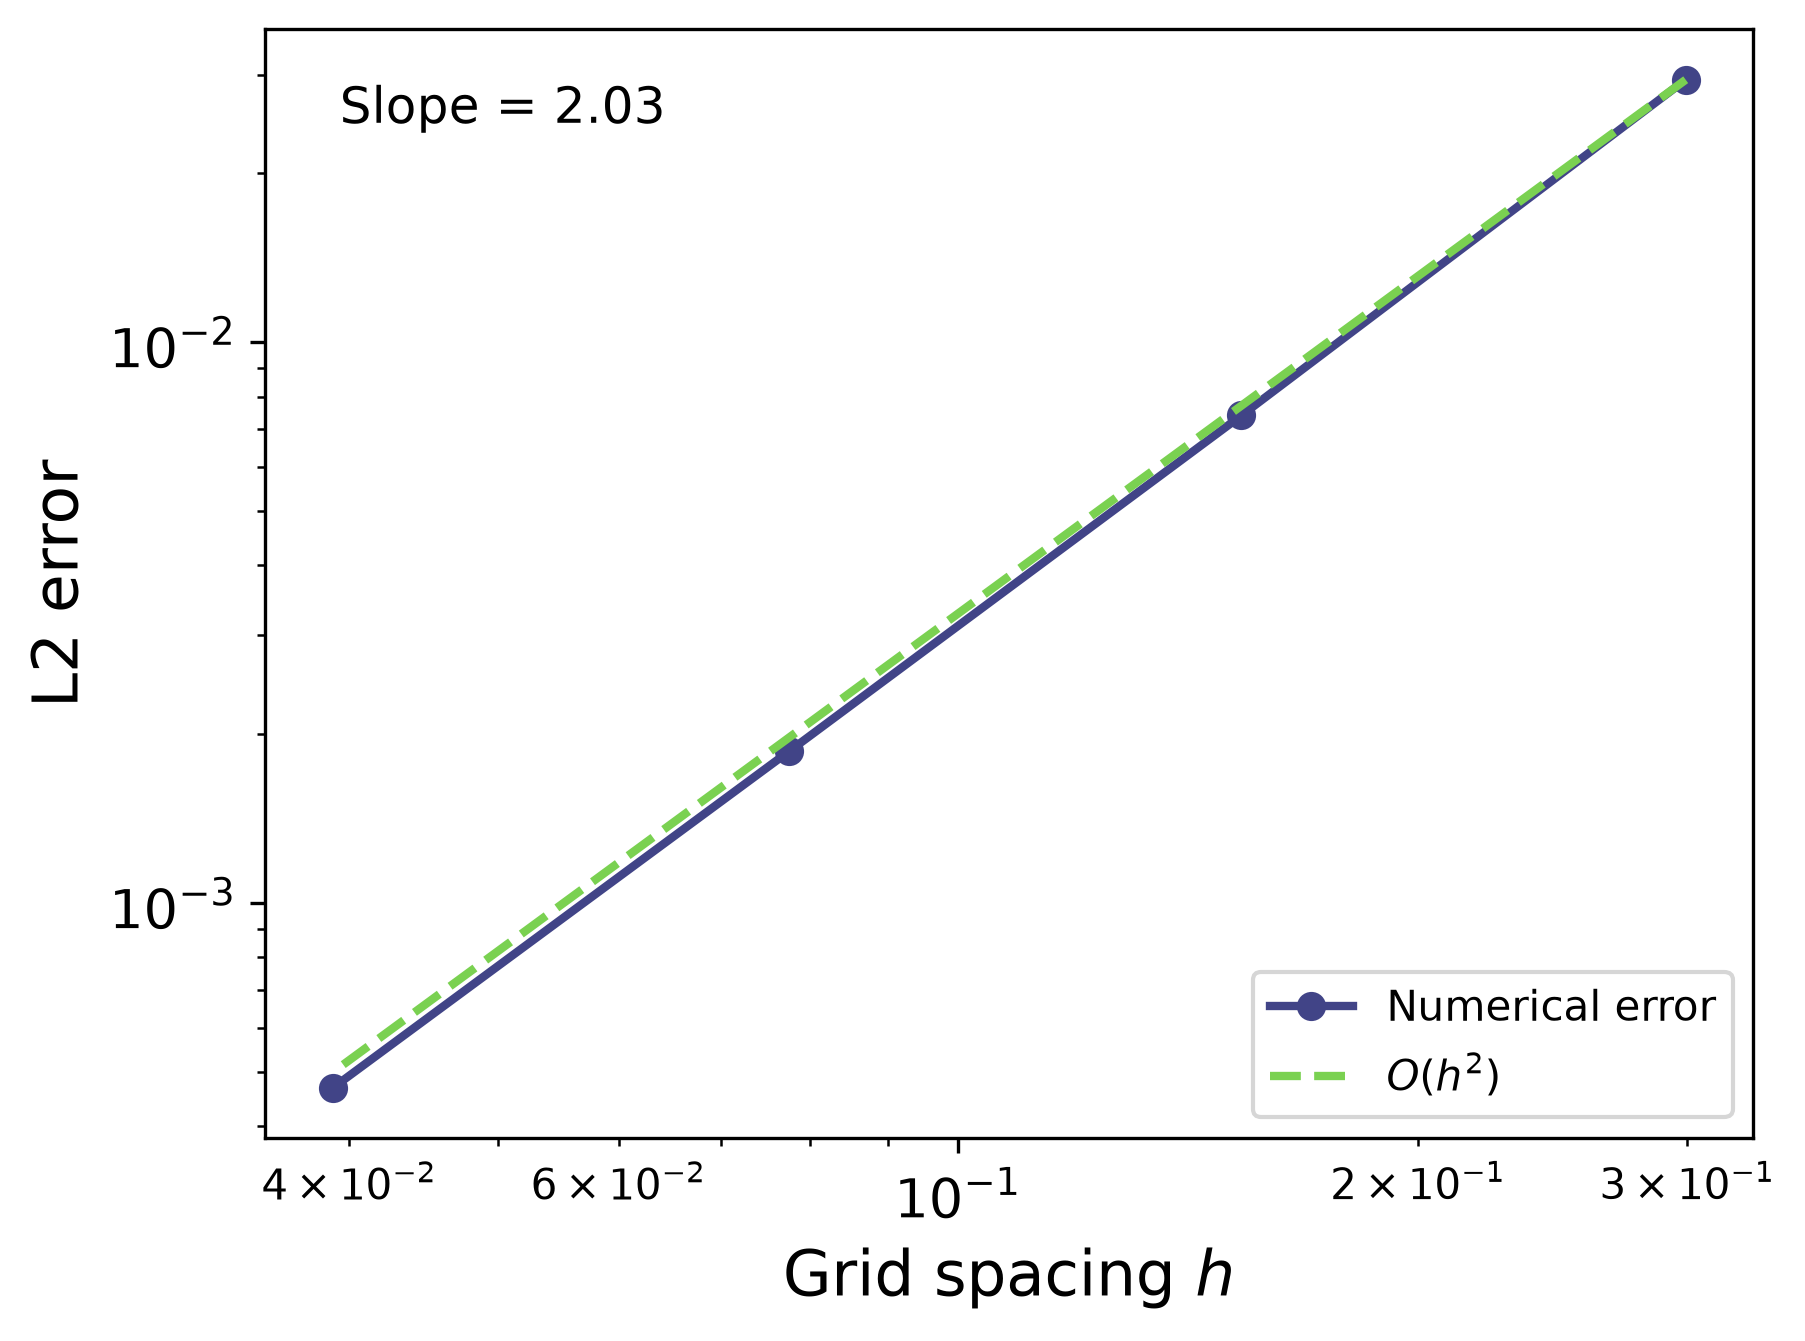
\includegraphics[width=0.75\textwidth]
{problem1_convergence.png}
\caption{Convergence of the finite-difference Poisson solver
compared with the theoretical $O(h^2)$ rate.}
\end{figure}

The relative $L^2$ error decreases as the grid size increases, indicating that the numerical solution converges to the exact solution. The observed convergence has a slope of 2.03, which matches the expected second-order accuracy. 

\begin{figure}[H]
\centering
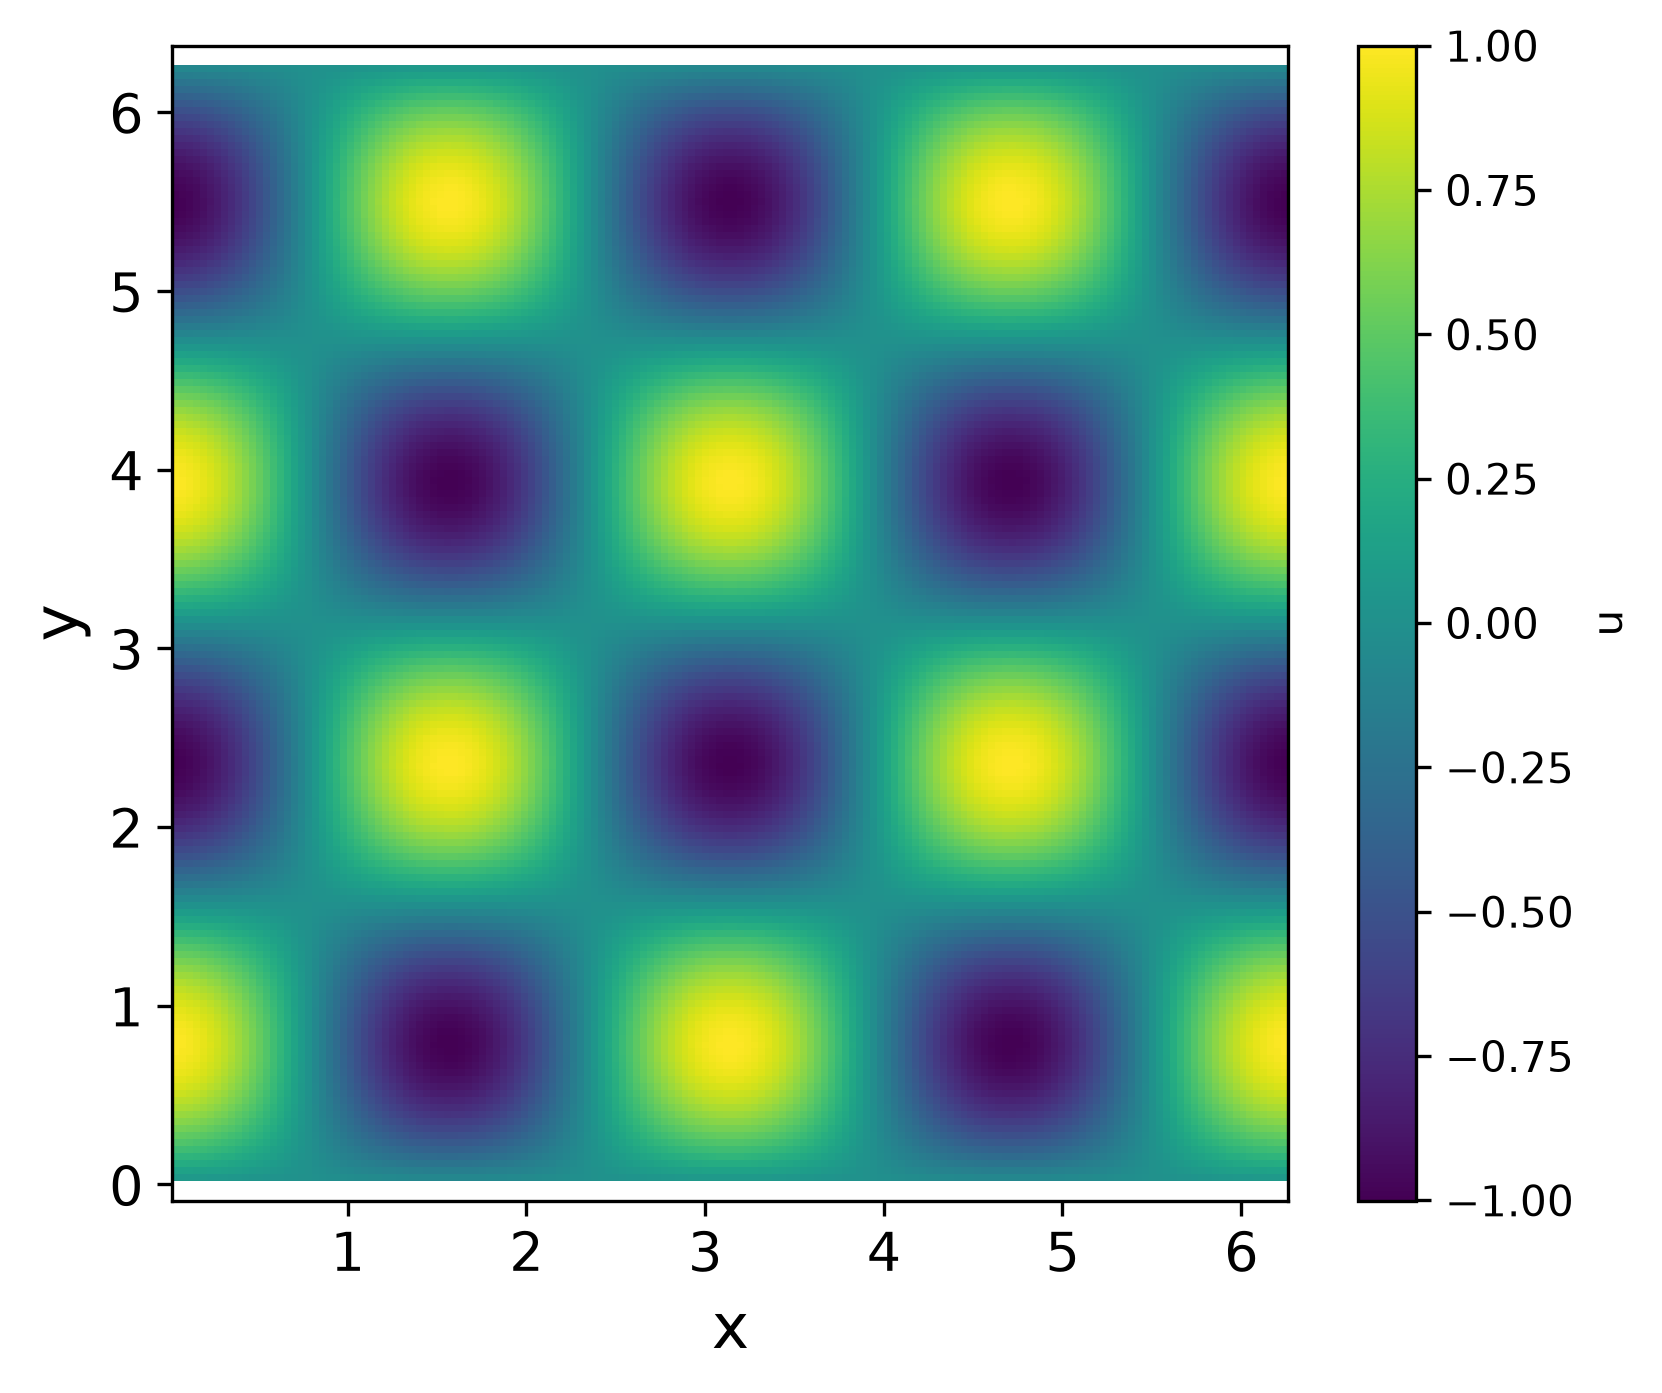
\includegraphics[width=0.65\textwidth]
{problem1_solution.png}
\caption{Numerical solution of the Poisson equation.}
\end{figure}

The numerical solution shows a sinusoidal pattern, which is expected since $u(x,y)=\cos(2x)\sin(2y)$. The small relative $L^2$ errors indicate that the finite-difference method accurately approximates the exact solution.

\newpage
% ==========================================================
\section*{Problem 2: Poisson Equation with an Immersed Boundary}
% ==========================================================

\textbf{Question.}
Consider the Poisson equation from Problem 1 with an additional Dirichlet boundary condition imposed along the circle
\[
x^{ib}=\pi+\cos\theta,\qquad
y^{ib}=\pi+\sin\theta,\qquad
0\leq\theta<2\pi.
\]
Prescribe
\[
u(x^{ib},y^{ib})
=\cos(2x^{ib})\sin(2y^{ib}).
\]

Discretize the immersed boundary using points spaced approximately one Cartesian grid spacing apart. Use a regularized two-dimensional Gaussian kernel with width $a=1.2h$ to construct spreading and interpolation operators. Formulate the saddle-point system and solve it using matrix-free GMRES. Investigate the convergence rate of the numerical solution under grid refinement, comparing it with the expected $O(h^{1.5})$ rate.

\subsection*{Solution}

The immersed boundary formula changes the Poisson equation into
\[
\nabla^2u=f(x,y)+S^{ib}(q),
\]
where $S^{ib}(q)$ is the spreading operation.

The immersed boundary is the circle
\[
x^{ib}=\pi+\cos\theta,
\qquad
y^{ib}=\pi+\sin\theta,
\]
and the Dirichlet value is
\[
u(x^{ib}, y^{ib})=\cos(2x^{ib})\sin(2y^{ib}).
\]

After rearranging all of the unknowns onto one side, we get the following saddle point system:
\[
\begin{bmatrix}
\nabla^2 & -S^{ib}\\
J^{ib} & 0
\end{bmatrix}
\begin{bmatrix}
u(x,y)\\q
\end{bmatrix}
=
\begin{bmatrix}
f(x,y)\\ \cos(2x^{ib})\sin(2y^{ib})
\end{bmatrix},
\]

Then, I discretized using the five-point finite-difference stencil and solved the resulting system using matrix-free GMRES, without explicitly forming the full saddle-point matrix.


\begin{table}[H]
\centering
\begin{tabular}{ccc}
\toprule
$N$ & IB Points & Relative $L^2$ Error\\
\midrule
20  & 21  & $3.035\times10^{-1}$\\
40  & 41  & $5.808\times10^{-2}$\\
80  & 81  & $1.408\times10^{-2}$\\
160 & 161 & $3.412\times10^{-3}$\\
\bottomrule
\end{tabular}
\caption{Relative $L^2$ error with increasing grid sizes.}
\end{table}


\begin{figure}[H]
\centering
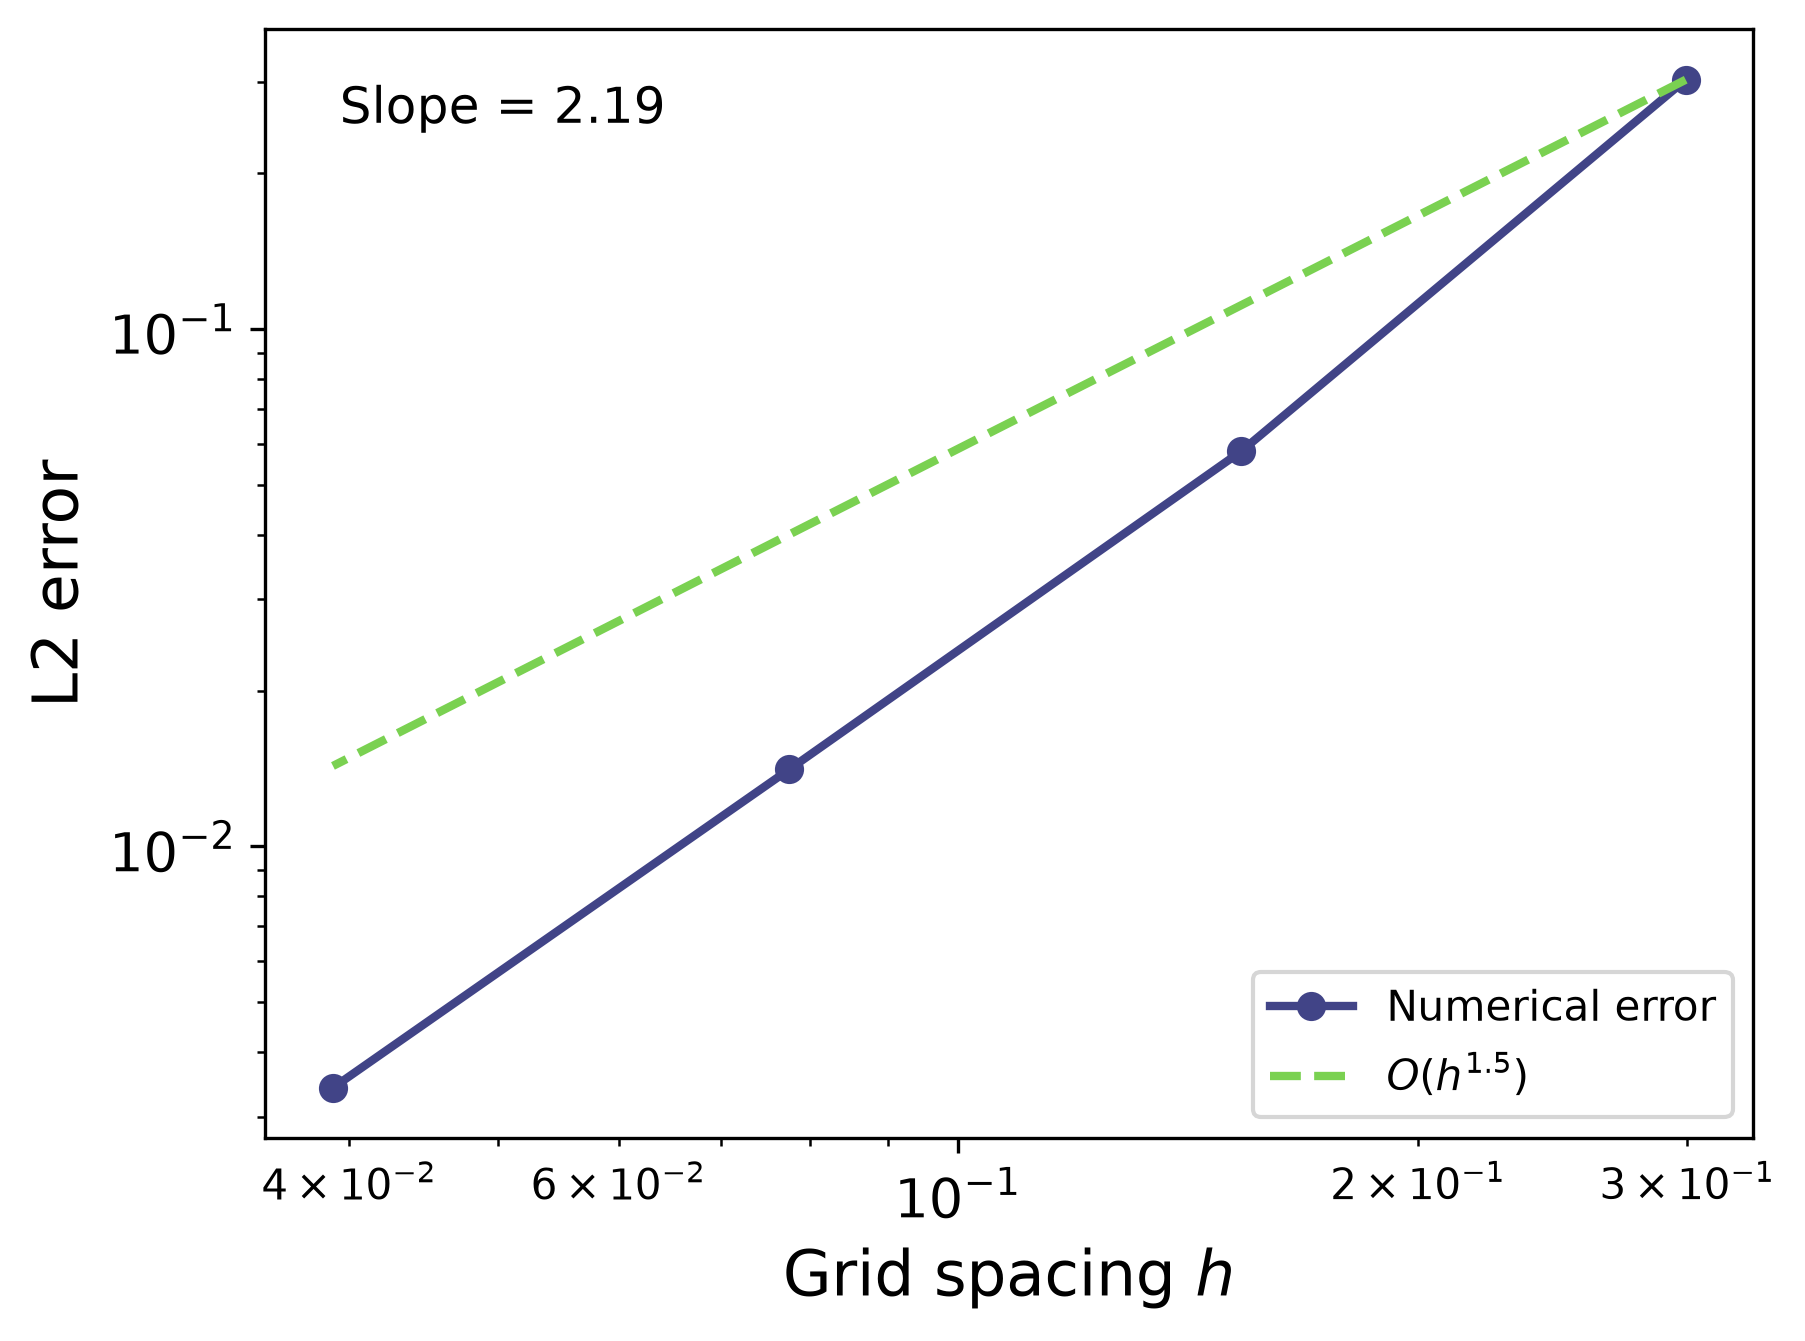
\includegraphics[width=0.75\textwidth]
{problem2_convergence.png}
\caption{Immersed boundary convergence compared with
the $O(h^{1.5})$ reference rate.}
\end{figure}


The relative $L^2$ error decreases as the grid size increases, but the observed convergence order is 2.19 which exceeds the expected order of 1.5. To investigate this difference, I compared the immersed boundary solution with the standard Poisson solution and got a convergence order of 2.18 for their relative difference. I also measured the Gaussian interpolation error against the exact solution and got an order of 1.89. These results suggest that the solution has approximately second-order accuracy, and I'm not sure why it's different from the expected accuracy of 1.5.

\begin{figure}[H]
\centering
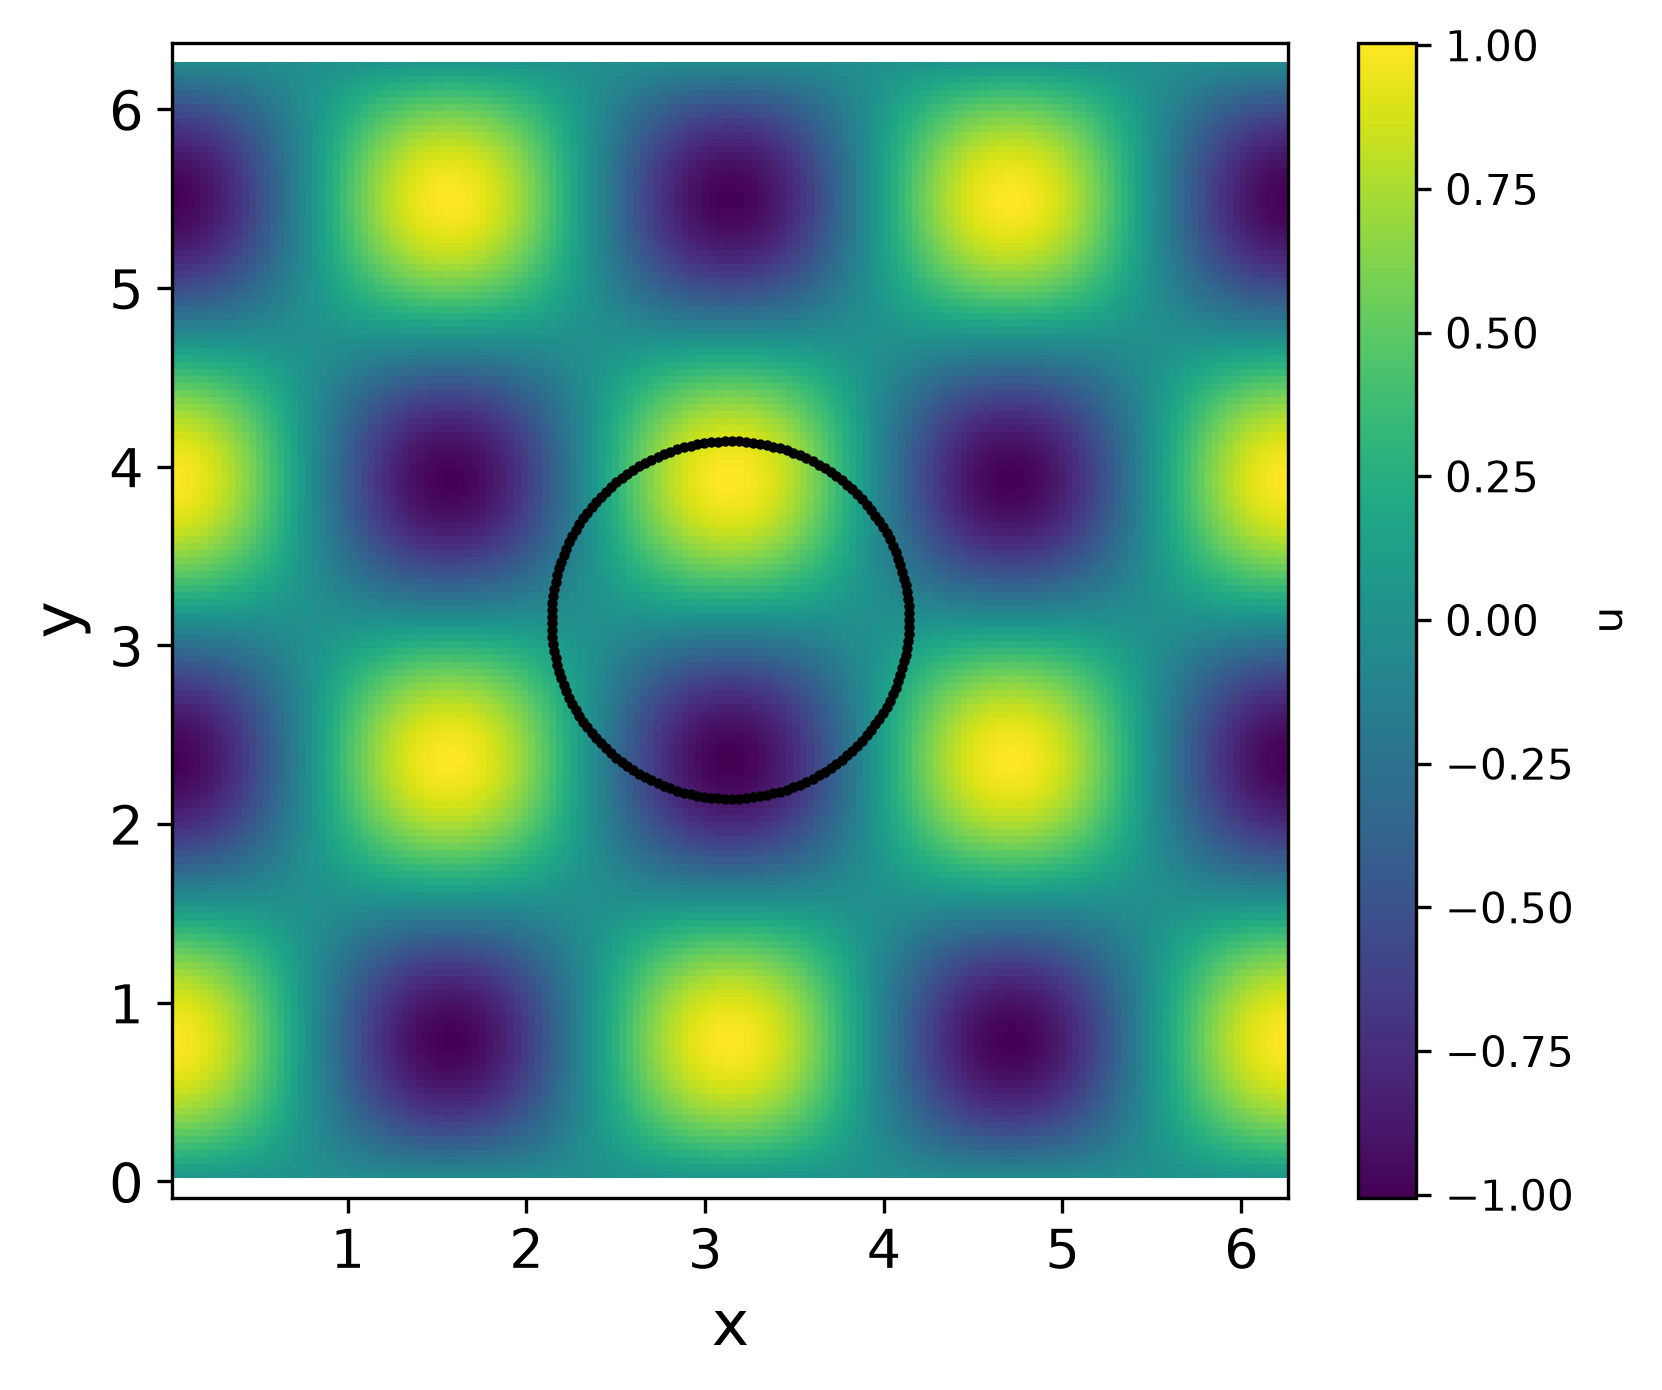
\includegraphics[width=0.65\textwidth]
{problem2_solution.png}
\caption{Numerical Poisson solution with the circular immersed boundary shown in black.}
\end{figure}

The numerical solution still shows the sinusoidal pattern from Problem 1 because the solution is very similar. The black points indicate the circular immersed boundary centered at $(\pi,\pi)$ with radius 1. The decreasing relative $L^2$ errors imply convergence.

\newpage
% ==========================================================
\subsection*{Problem 2(a): Immersed Boundary Point Spacing}
% ==========================================================

\textbf{Question.}
Investigate how the spacing between immersed boundary
points affects numerical accuracy and computational
speed. Compare spacings of $0.5h$, $h$, $2h$, and $4h$.
Explain what happens when the immersed boundary points
are much closer together or farther apart than the
Cartesian grid spacing.

\subsubsection*{Solution}

To investigate the effect of immersed boundary spacing, I fixed the Cartesian grid at $N=40$ and varied the spacing between immersed boundary points from $0.5h$ to $4h$.

\begin{table}[H]
\centering
\small
\begin{tabular}{ccccc}
\toprule
Spacing & IB Points & Relative $L^2$ Error
& Time (s) & GMRES Info\\
\midrule
$0.5h$ & 82 & $7.296\times10^{-1}$ & 0.20 & 0\\
$h$    & 41 & $5.808\times10^{-2}$ & 0.03 & 0\\
$2h$   & 20 & $5.803\times10^{-2}$ & 0.02 & 0\\
$4h$   & 10 & $5.666\times10^{-2}$ & 0.02 & 0\\
\bottomrule
\end{tabular}
\caption{Effect of immersed boundary point spacing on relative $L^2$ error and computational time for $N=40$. GMRES info = 0 indicates successful convergence.}
\end{table}

The relative $L^2$ error remains approximately 0.058 for immersed boundary spacings of $h$, $2h$, and $4h$. However, decreasing the spacing to $0.5h$ relatively increases the error to approximately 0.730, suggesting that increasing the number of immersed boundary points does not necessarily improve accuracy.

GMRES converged successfully for all four spacings. The $0.5h$ case required the longest runtime at 0.20 seconds.

\newpage
% ==========================================================
\section*{Problem 3: An Almost Minimal Surface}
% ==========================================================

\textbf{Question.}
Use the immersed boundary method from Problem 2
to solve
\[
\nabla^2u=S^{ib}(q)
\]
on $[0,2\pi]^2$, with homogeneous Dirichlet boundary
conditions on the outer square:
\[
u(0,y)=u(2\pi,y)=u(x,0)=u(x,2\pi)=0.
\]

Use the same circular immersed boundary,
\[
x^{ib}=\pi+\cos\theta,\qquad
y^{ib}=\pi+\sin\theta,
\]
and prescribe
\[
u(x^{ib},y^{ib})
=\cos(2x^{ib})\sin(2y^{ib}).
\]
Plot the resulting numerical surface and compare it
with the reference figure in the assignment.

\subsection*{Solution}

For this problem, we solve
\[
\nabla^2u=S^{ib}(q),
\]
with homogeneous Dirichlet conditions on the outer square. The distributed forcing function is zero, so the solution is driven entirely by the immersed boundary source strengths. 

Using the same circular immersed boundary, the numerical solution is computed using $N=60$. GMRES converged successfully, and the solution and convergence plots are below.

\begin{figure}[H]
\centering
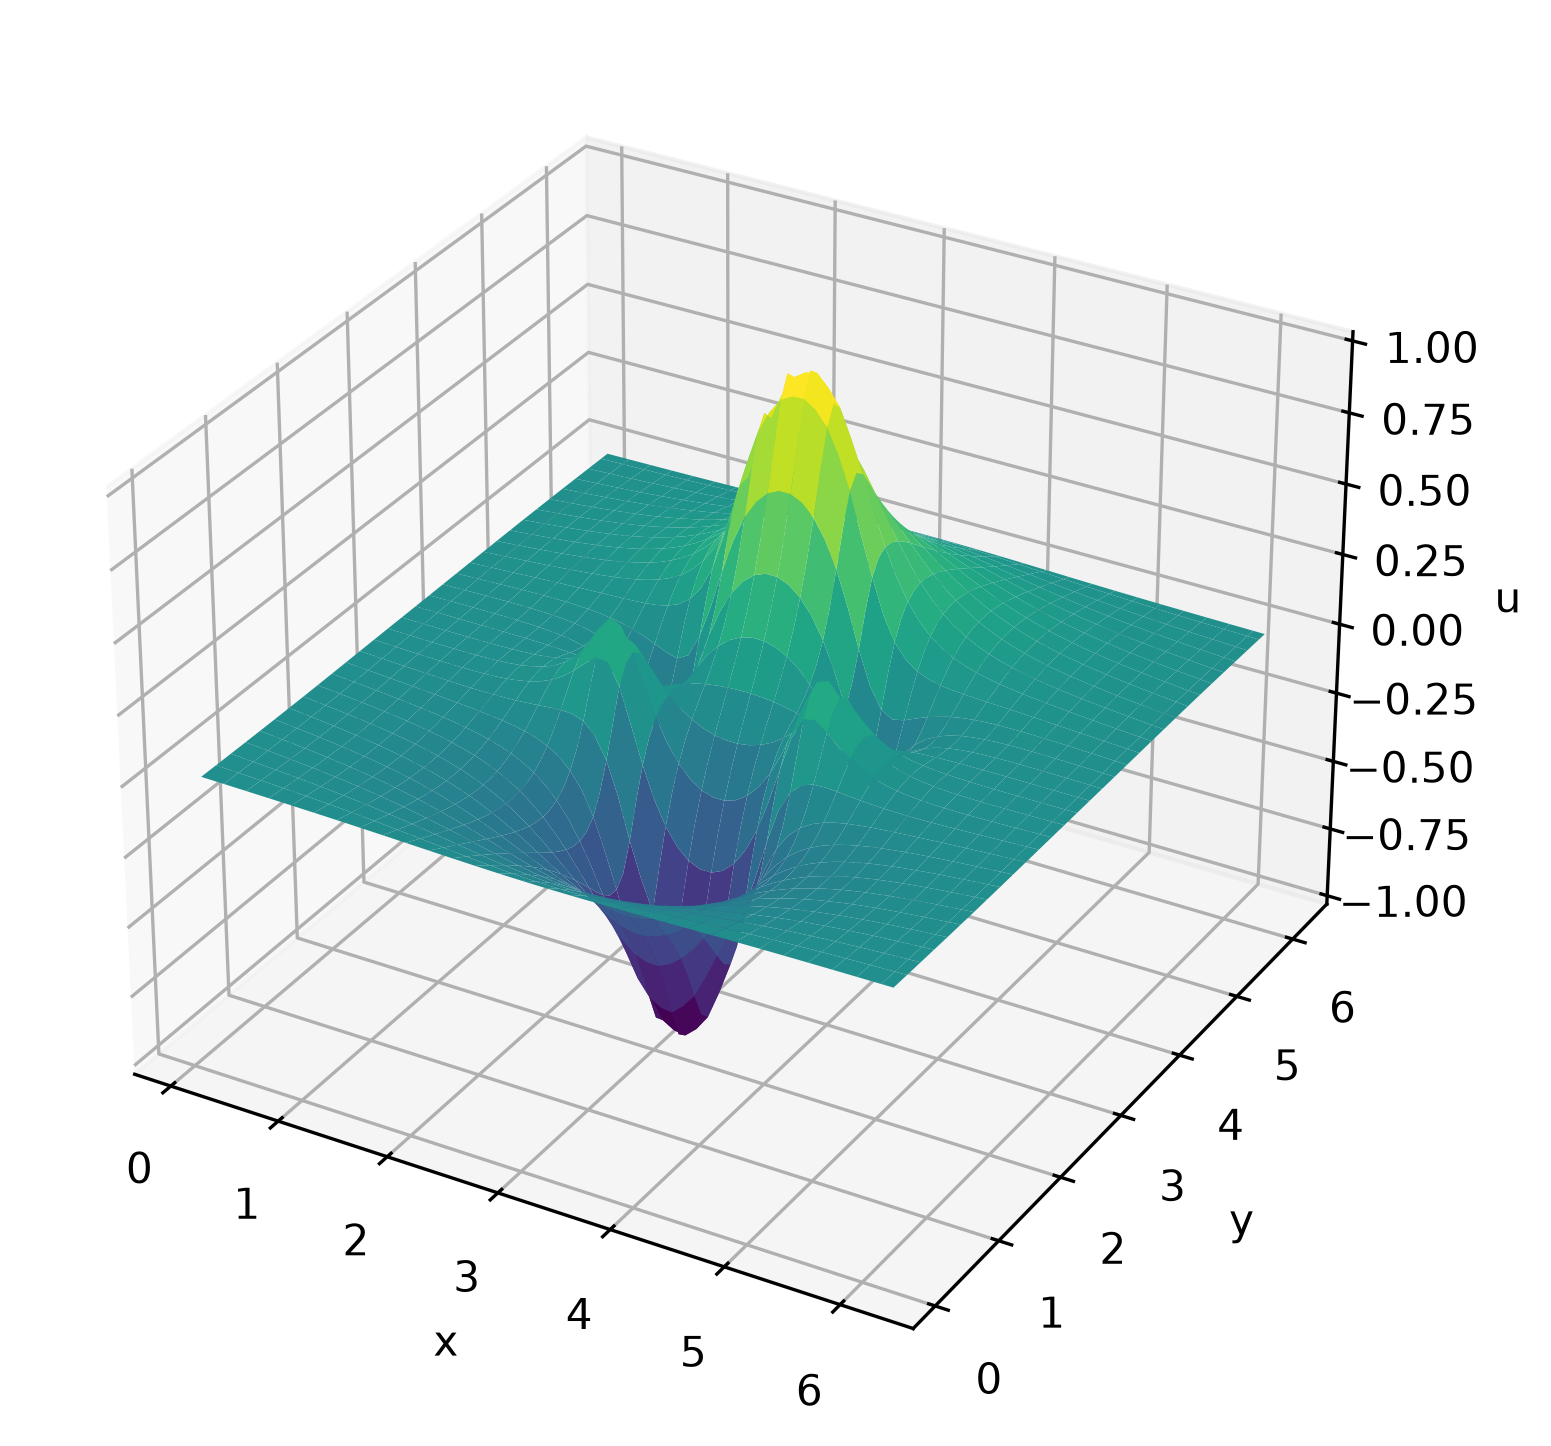
\includegraphics[width=0.85\textwidth]
{problem3_surface.png}
\caption{Three-dimensional numerical solution of
the almost-minimal-surface problem.}
\end{figure}

The three-dimensional solution shows a positive peak and a negative peak near the immersed boundary, corresponding to the Dirichlet conditions. Unlike Problems 1 and 2, the solution does not show a sinusoidal pattern because the distributed forcing is zero. The solution is driven by the immersed boundary sources and approaches zero toward the outer boundaries.

\begin{figure}[H]
\centering
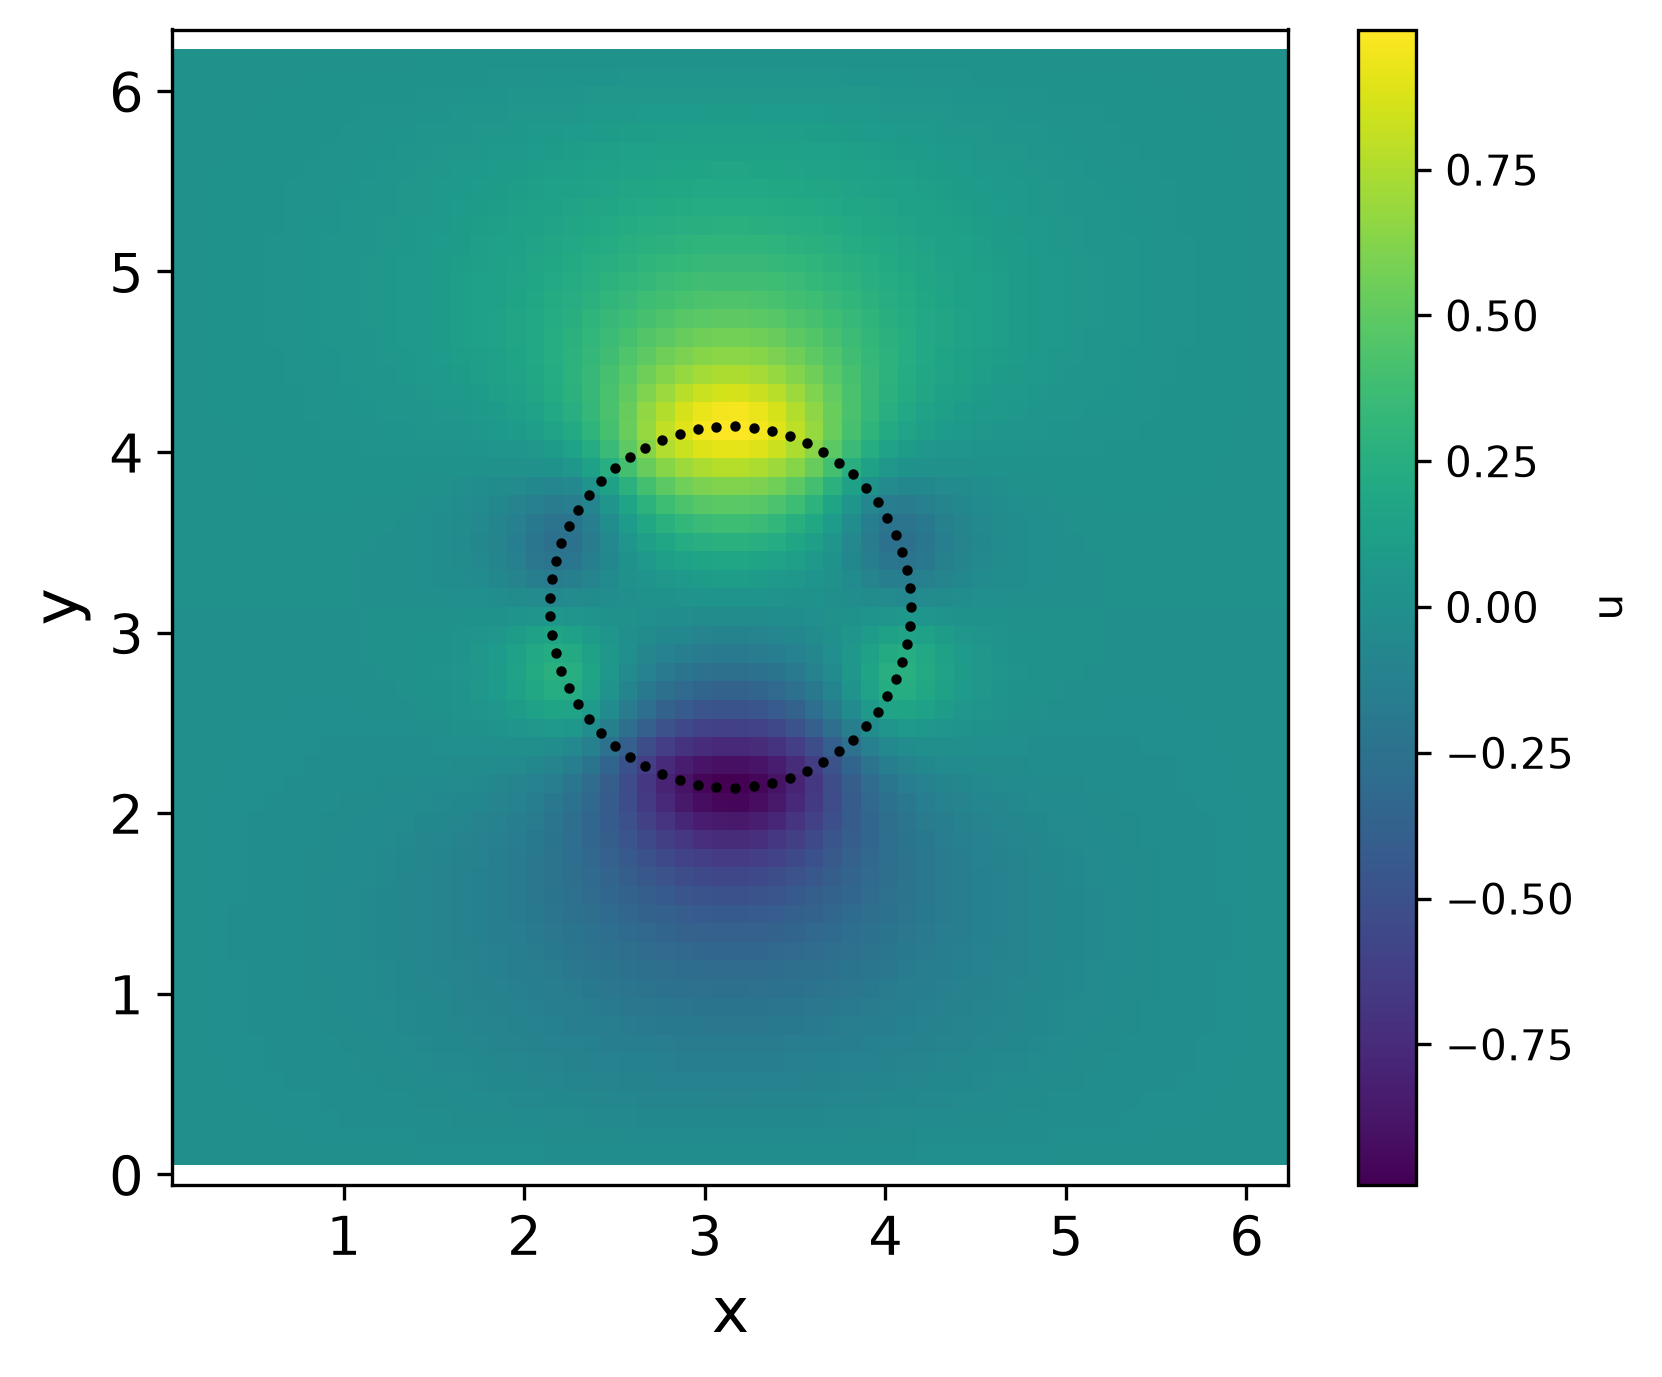
\includegraphics[width=0.65\textwidth]
{problem3_solution.png}
\caption{Top view of the numerical solution with
the immersed boundary marked in black.}
\end{figure}

The two-dimensional plot shows localized regions of positive and negative values near the immersed circle. The solution becomes smaller farther from the circle, consistent with the Dirichlet conditions on the outer square. 

\newpage
% ==========================================================
\section*{Problem 4: Charlie's Rule}
% ==========================================================

\textbf{Question.}
Play with the code!

\subsection*{Solution}

For this extension, I changed the immersed boundary geometry by replacing the single circle with two smaller circles. Both circles have radius $0.5$ and are centered at $(2,\pi)$ and $(4,\pi)$, respectively. I then
solved the same equation as in Problem 3,
\[
\nabla^2 u = S^{ib}(q),
\]
with homogeneous Dirichlet conditions on the outer boundary and prescribed values
$u(x^{ib},y^{ib})=\cos(2x^{ib})\sin(2y^{ib})$
on both immersed circles.

\begin{figure}[H]
    \centering
    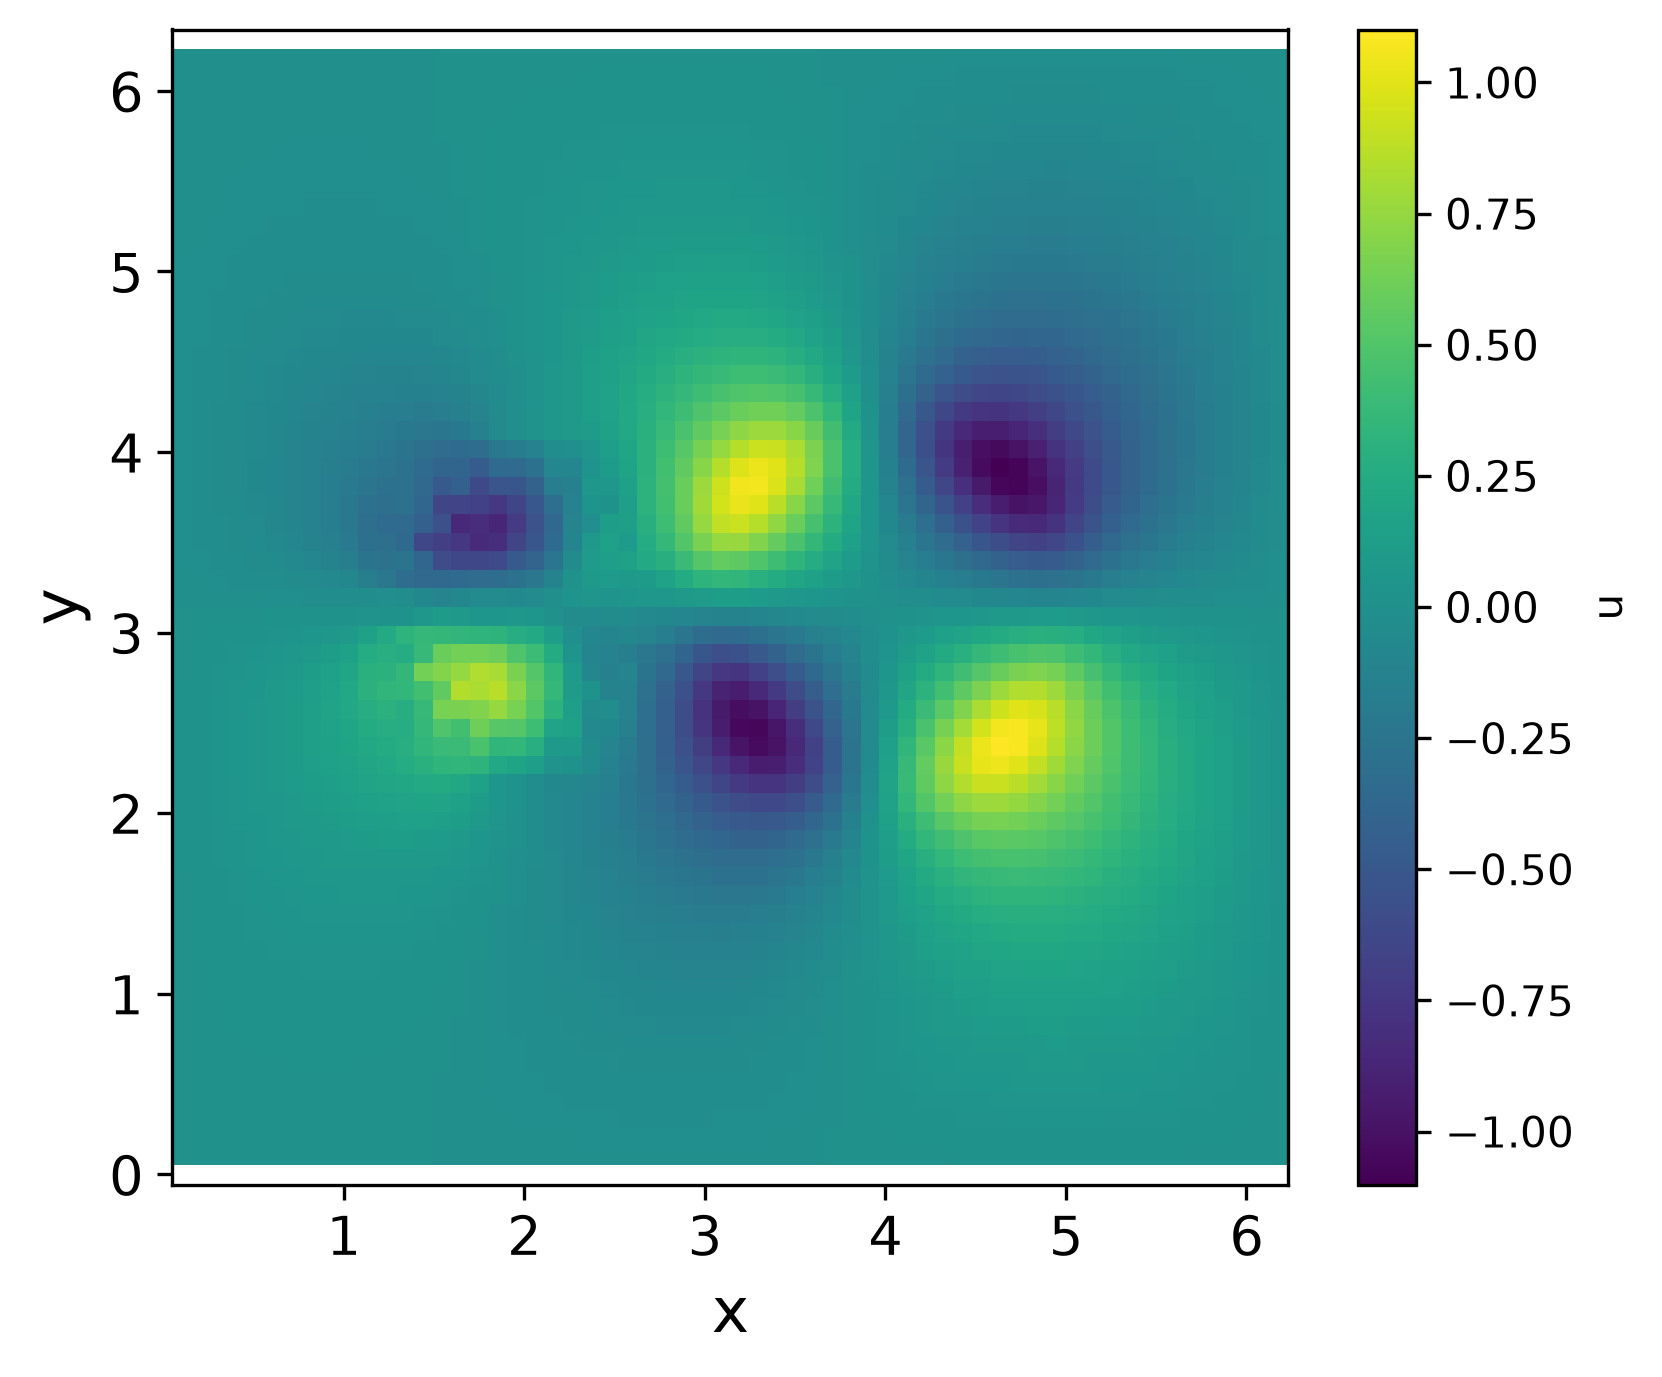
\includegraphics[width=0.75\textwidth]
    {problem4_solution.png}
    \caption{Numerical solution with two circular
    immersed boundaries.}
\end{figure}

\begin{figure}[H]
    \centering
    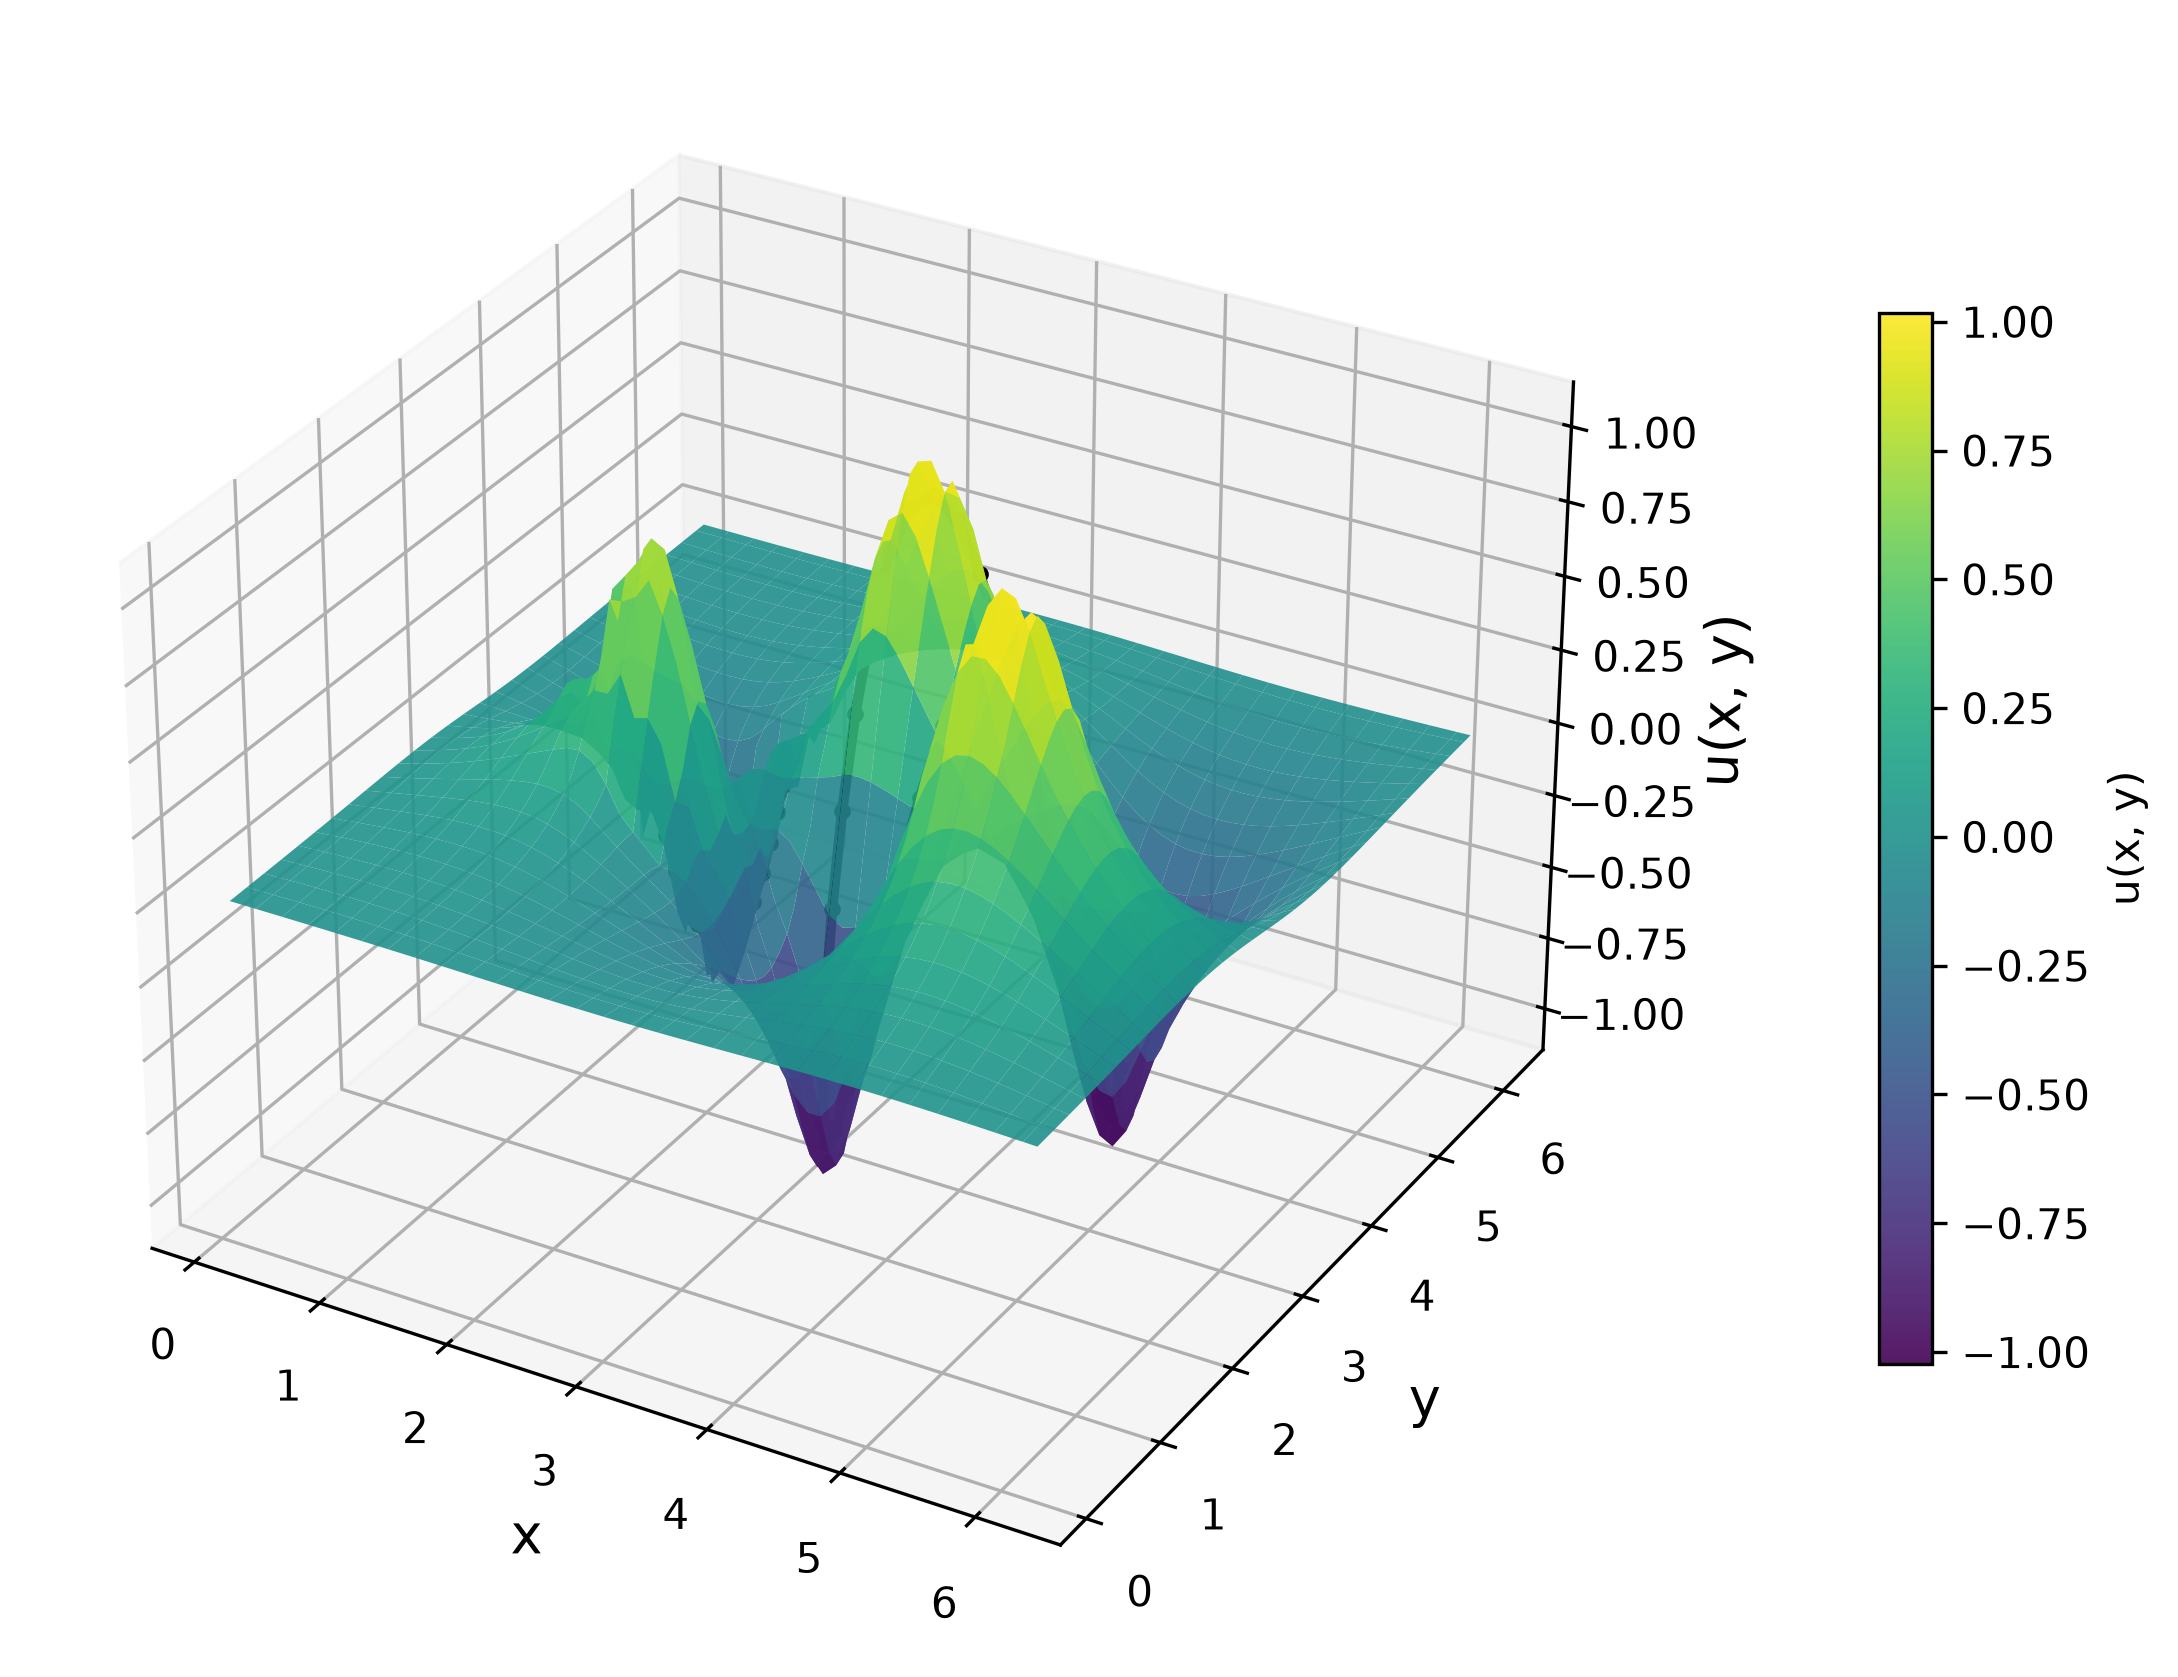
\includegraphics[width=0.85\textwidth]
    {problem4_surface.png}
    \caption{Three-dimensional numerical solution with
    two circular immersed boundaries.}
\end{figure}

This experiment shows that the immersed boundary method can accommodate multiple internal boundaries. I thought it was interesting that I could create a different surface just by changing the locations and shapes of the immersed boundaries, without having to change the solver itself. Adding a second circle creates a more complicated surface, with the two boundaries influencing the solution around each other. 

\end{document}
